%---------------------------------------------------------------------------%
%->> Backmatter
%---------------------------------------------------------------------------%
%->> Question
%---------------------------------------------------------------------------%
\lecture{Research Presentation}{lec_present_question}
%---------------------------------------------------------------------------%
{%
\begin{frame}[plain]
    \begin{center}
        {\large\bfseries {\enorcn{Thank you for your attention!}{感谢聆听!\par\medskip 敬请批评指正}}}
    \end{center}
    \tikzart[t=p,x=0,y=-4,w=4]{logo_uw}
    \addtocounter{framenumber}{-1}% modify the counter to exclude a frame from total count
\end{frame}
}
%---------------------------------------------------------------------------%
%->> Appendix
%---------------------------------------------------------------------------%
\lecture{Research Presentation}{lec_present_appendix}
%---------------------------------------------------------------------------%
\appendix% begin appendix
%\newcounter{finalframe}% define a new counter
%\setcounter{finalframe}{\value{framenumber}}% save regular slides counter
%---------------------------------------------------------------------------%
\section{\appendixname}% the end page.
\frame{\tableofcontents}% outline for appendix
%---------------------------------------------------------------------------%
\subsection{\enorcn{Classic Beamer Style}{常规Beamer风格}}
%---------------------------------------------------------------------------%
\begin{frame}[fragile]
    \frametitle{Sod's problem \parencite{sod1978survey}}

    \begin{columns}
        \begin{column}{.40\textwidth}
            \centering
            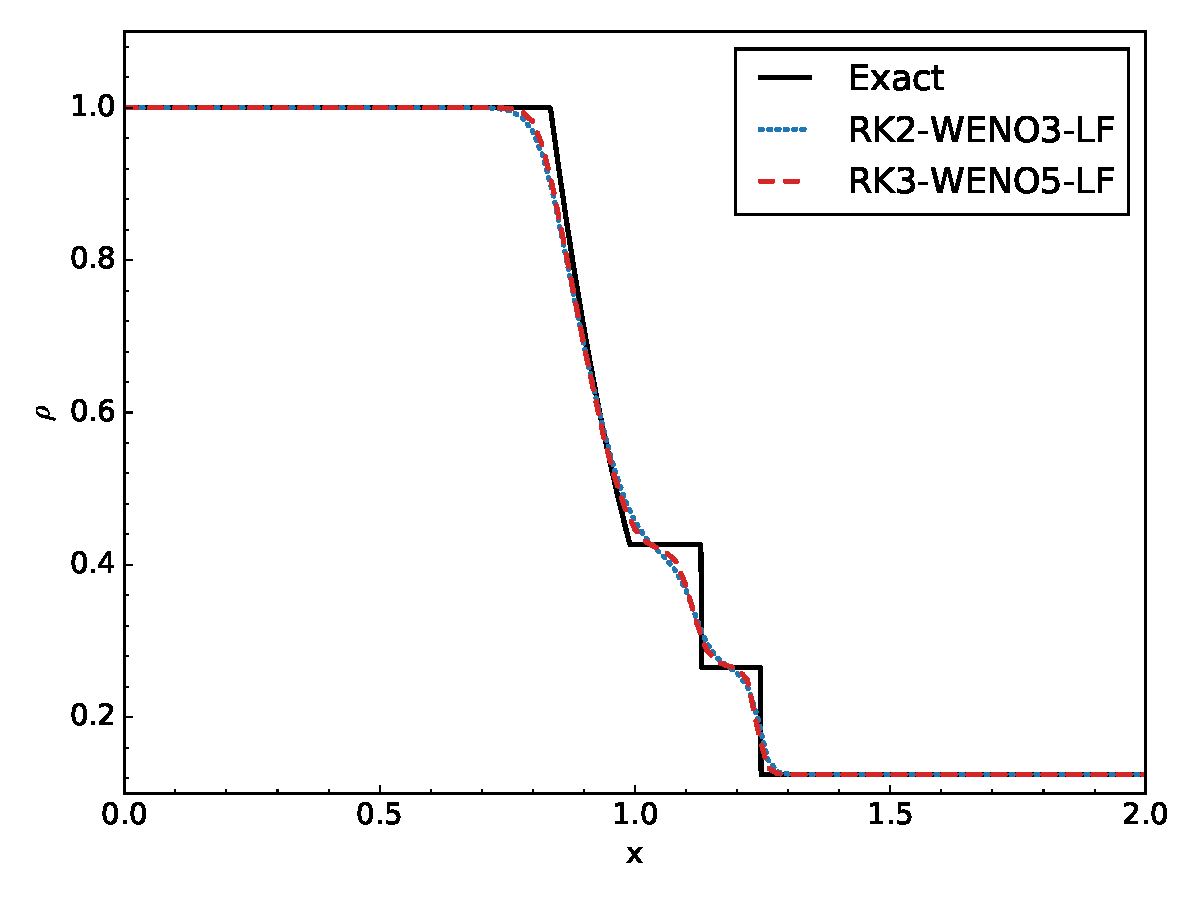
\includegraphics[width=\textwidth]{riemann_1d_sod_rho_x_n100}

            {$n=100$}
        \end{column}

        \begin{column}{.40\textwidth}
            \centering
            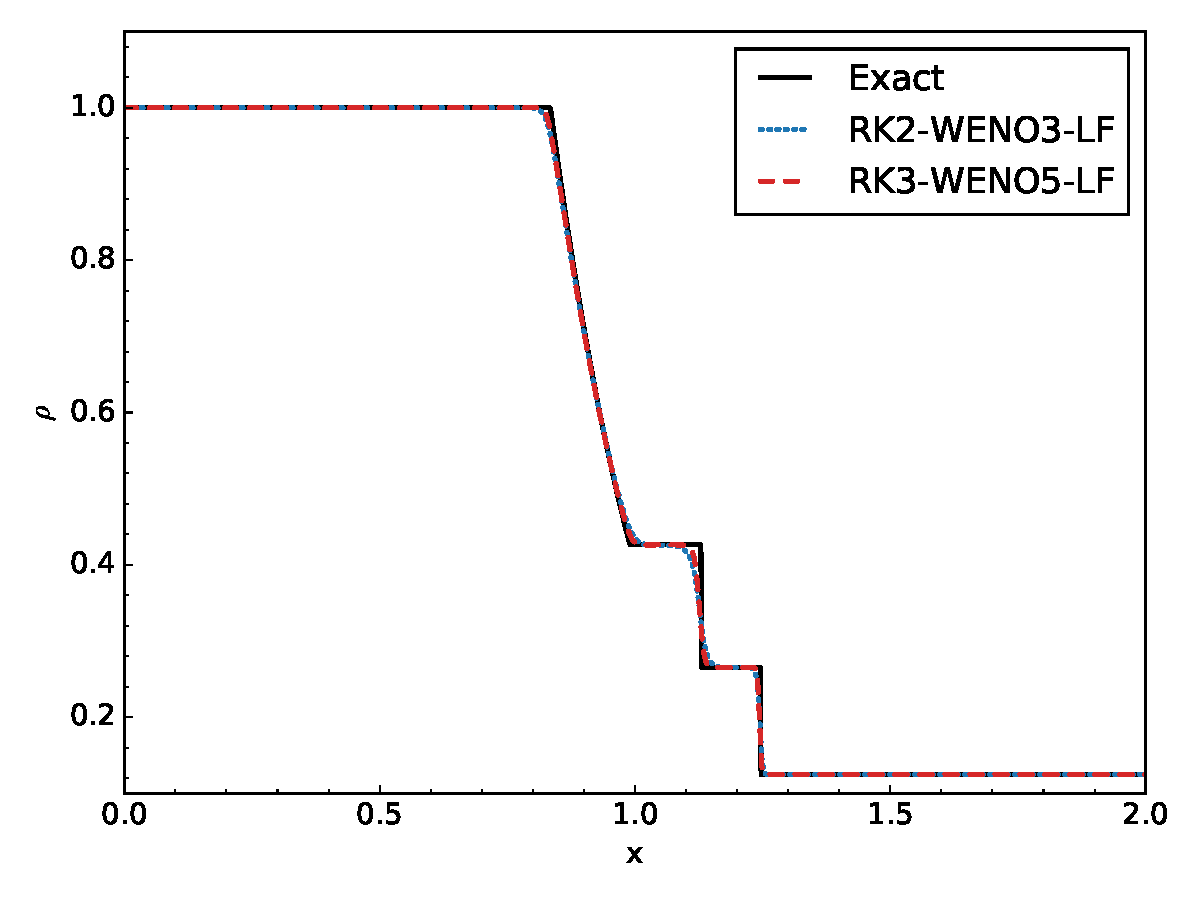
\includegraphics[width=\textwidth]{riemann_1d_sod_rho_x_n500}

            {$n=500$}
        \end{column}
    \end{columns}

    \bigskip\vfill

    \[
        \begin{gathered}
            \begin{aligned}
                \rho &= 1; & u &= 0; & p &= 1 & \ \text{if}\ & 0 \le x < 1 \\
                \rho &= 0.125; & u &= 0; & p &= 0.1 & \ \text{if}\ & 1 < x \le 2
            \end{aligned}
        \end{gathered}
    \]
\end{frame}
%---------------------------------------------------------------------------%
\lecture{Research Presentation}{lec_present_ref}
%---------------------------------------------------------------------------%
\subsection{\enorcn{References}{参考文献}}
%---------------------------------------------------------------------------%
\begin{frame}[allowframebreaks]
    \frametitle{References}
    \printbibliography[heading=none]%
\end{frame}
%---------------------------------------------------------------------------%
%\setcounter{framenumber}{\value{finalframe}}% rectify the slides counter
%---------------------------------------------------------------------------%
